%%
%% Keyboard keys.
%%
%
\RequirePackage[os=win]{menukeys}%
\renewmenumacro{\keys}[+]{roundedkeys}%
\renewmenumacro{\directory}[/]{hyphenatepaths}%
%
%% Get the Windows and Apple Macintosh symbols.
%% see https://tex.stackexchange.com/questions/387952
\RequirePackage{fontawesome}%
\tw@make@key@box{OS@mac}{\faApple}%
\tw@make@key@box{OS@win}{\faWindows}%
\tw@make@key@macro*{\OS}%
%
%% The key sequence needed to launch a terminal under Ubuntu Linux.
\protected\gdef\ubuntuTerminal{\keys{\ctrl+\Alt+T}}%
%% The key sequence needed to launch a terminal under Microsoft Windows.
\protected\gdef\windowsTerminal{press \keys{\OSwin + R}, type in \textil{cmd}, and hit \keys{\return}}%
%
%% insert a icon button
\protected\gdef\@key@icon@button#1{\raisebox{-0.111111em}{\includegraphics[width=1em,height=1em,keepaspectratio]{\bookbaseDir/graphics/icons/#1}}}
%
%% The PyCharm main menu key
\protected\gdef\pycharmMainMenu{\ensuremath{\mathrel{\rlap{\raisebox{\fontdimen22\textfont2}{\ensuremath{=}}}\raisebox{-0.5\fontdimen22\textfont2}{\ensuremath{=}}}}}
\global\let\pgmodelerMainMenu\pycharmMainMenu%
%% The PyCharm python console menu key
\protected\gdef\pycharmConsole{\@key@icon@button{pycharmPythonConsole}}%
%% The pycharm debugger resume command
\protected\gdef\pycharmDebuggerResume{\@key@icon@button{pycharmDebuggerResumeProgram}}%
%% The pycharm debugger step over command
\protected\gdef\pycharmDebuggerStepOver{\@key@icon@button{pycharmDebuggerStepOver}}%
%% The PyCharm errors symbol
\protected\gdef\pycharmErrorsSymbol{\@key@icon@button{pycharmErrorsSymbol}}%
%% The PyCharm errors button
\protected\gdef\pycharmErrorsButton{\@key@icon@button{pycharmErrorsButton}}%
%% The PyCharm warnings symbol
\protected\gdef\pycharmWarningsSymbol{\@key@icon@button{pycharmWarningsSymbol}}%
%% The PyCharm run button
\protected\gdef\pycharmRun{\@key@icon@button{pycharmRun}}%
%
% The LibreOffice Base refresh key button
\protected\gdef\libreOfficeBaseRefresh{\@key@icon@button{libreOfficeBaseRefresh}}%
% The LibreOffice Base key button
\protected\gdef\libreOfficeBaseKey{\@key@icon@button{libreOfficeBaseKey}}%
% The LibreOffice Base design mode button
\protected\gdef\libreOfficeBaseDesignMode{\@key@icon@button{libreOfficeBaseDesignMode}}%
% The LibreOffice Base more button
\protected\gdef\libreOfficeBaseMore{\@key@icon@button{libreOfficeBaseMore}}%
% The LibreOffice Base table button
\protected\gdef\libreOfficeBaseTable{\@key@icon@button{libreOfficeBaseTable}}%
% The LibreOffice PDF button
\protected\gdef\libreOfficePdf{\@key@icon@button{libreOfficePdf}}%
%
%% The four different Crow's Foot end notations.
\protected\gdef\crowsFootOptionalOne{%
\raisebox{-0.111111em}{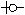
\includegraphics[height=0.93em,keepaspectratio]{\bookbaseDir/graphics/icons/crowsFootOptionalOne}}}%
\protected\gdef\crowsFootMandatoryOne{%
\raisebox{-0.111111em}{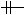
\includegraphics[height=0.93em,keepaspectratio]{\bookbaseDir/graphics/icons/crowsFootMandatoryOne}}}%
\protected\gdef\crowsFootOptionalMany{%
\raisebox{-0.111111em}{
\includegraphics[height=0.93em,keepaspectratio]{\bookbaseDir/graphics/icons/crowsFootOptionalMany}}}%
\protected\gdef\crowsFootMandatoryMany{%
\raisebox{-0.111111em}{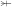
\includegraphics[height=0.93em,keepaspectratio]{\bookbaseDir/graphics/icons/crowsFootMandatoryMany}}}%
%
\edef\@@crowsfoot@oo{\detokenize{O1}}%
\edef\@@crowsfoot@mo{\detokenize{M1}}%
\edef\@@crowsfoot@om{\detokenize{OM}}%
%
%% Crow's foot notation for entity relationship diagrams
%% #1 first label (left side)
%% #2 first end of relationship (left side)
%% #3 second label (right side)
%% #4 second relationship end (right side)
%% relationship ends are: O1 = optional 1, M1 = mandatory 1,
%%                        OM = optional many, MM = mandatory many
\protected\gdef\crowsFoot#1#2#3#4{\mbox{%
#1%
\edef\@crowf@img@a{\detokenize{#2}}%
\ifx\@crowf@img@a\@@crowsfoot@oo\let\@crowf@img@a\crowsFootOptionalOne%
\else\ifx\@crowf@img@a\@@crowsfoot@mo\let\@crowf@img@a\crowsFootMandatoryOne%
\else\ifx\@crowf@img@a\@@crowsfoot@om\let\@crowf@img@a\crowsFootOptionalMany%
\else\let\@crowf@img@a\crowsFootMandatoryMany%
\fi\fi\fi%
\edef\@crowf@img@b{\detokenize{#4}}%
\ifx\@crowf@img@b\@@crowsfoot@oo\let\@crowf@img@b\crowsFootOptionalOne%
\else\ifx\@crowf@img@b\@@crowsfoot@mo\let\@crowf@img@b\crowsFootMandatoryOne%
\else\ifx\@crowf@img@b\@@crowsfoot@om\let\@crowf@img@b\crowsFootOptionalMany%
\else\let\@crowf@img@b\crowsFootMandatoryMany%
\fi\fi\fi%
\hspace*{0.1em}%
\@crowf@img@a%
\hspace*{-0.25em}%
\reflectbox{\@crowf@img@b}%
\hspace*{0.1em}%
#3%
}}%
%
